\section{Vraag \& Aanbod}

\subsection{Marktevenwicht}

`\textit{Hoe ontstaat een prijs in een markteconomie?}'. We gaan hier even vanuit dat er \entry{prijsnemerschap} is (de individu's kunnen de prijs niet be\"invloeden), en dat de producten \entry{homogeen} zijn (ze zijn allemaal gelijk, perfect inwisselbaar).\\

\par De \term{vraag}\footnote{Een uitdrukking van de marginale betalingsbereidheid.} naar de homogene producten wordt voorgesteld door een functie, de \entry{algemene vraagfunctie} $Q_x^v=f(P_x,P_{sub},P_{com},Y_{cap},\#\text{cons},\text{pref},t, ...)$. $P_x,P_{sub},Y_{cap}, ...$ zijn factoren die de vraag be\"invloeden. $P_x$ is bijvoorbeeld de prijs van het gevraagde product. $P_{sub}$ is de prijs van een vervangingsproduct (een \entry{substitutieproduct}). $P_{com}$ is de prijs van een \entry{complementair product} (een product dat gewoonlijk wordt gekocht met het gevraagde product, zoals frituurolie met aardappelen).
\par Met zo veel factoren zou de functie ingewikkeld worden. We kijken daarom naar de \entrystyled{partiele vraagfunctie}{parti\"ele vraagfunctie} : die vraagfunctie waarbij de factoren op \'e\'en factor na gelijk blijven\footnote{We redeneren \entry{ceteris paribus}.}. We kijken bijvoorbeeld naar de parti\"ele vraag in functie van de prijs van het gevraagde product, $Q_x^v=f(P_x\ |\ P_{sub}, P_{com}, Y_{cap}, \#cons, pref, t, ...)$. Een resultaat zie je in figuur \ref{fig:h2-vraagfunctie}. Merk op dat in de economie gewoonlijk de assen worden omgewisseld (de prijs $P_x$ zit dus op de y-as).

\begin{figure}[H]
\vspace{0.5cm}
\centering\small
\captionsetup{justification=centering,margin=2cm}
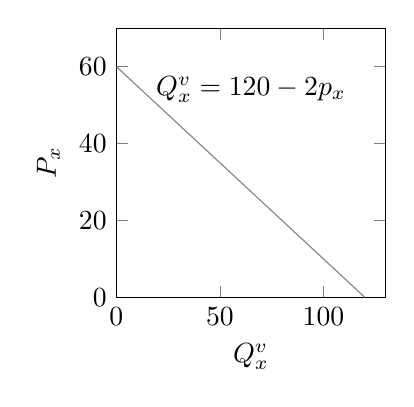
\begin{tikzpicture}
	\begin{axis}[name=left,xlabel=$Q_x^v$, ylabel=$P_x$, ymin=0, xmin=0, xmax=130, ymax=70,width=5cm, height=5cm]
		\addplot[gray, samples=120, domain=0:120] {60-(1/2)*x};
		\draw (axis cs:65,60) node[below]{$Q_x^v=120-2p_x$};
	\end{axis}
\end{tikzpicture}
\caption{Een parti\"ele vraagfunctie van een product $x$ bij varierende prijs $P_x$}
\label{fig:h2-vraagfunctie}
\end{figure}

De helling is \textit{negatief} : als de prijs daalt met $5$, dan stijgt de gevraagde hoeveelheid met $2*5$.
\par De functie kan men ook inverteren : $Q_x^v=120-2p_x$ (\textit{algemeen gevraagde hoeveelheid in functie van de prijs}) wordt dan $p_x=60-0,5Q_x^v$ (\textit{de prijs in functie van de algemeen gevraagde hoeveelheid}). Dit laatste kan ook geschreven worden als $MMB_x=60-0,5Q_x^c$, waarbij $Q_x^c$ de gevraagde hoeveelheid is van de consument. Het is immers de prijs die hij bereid is te betalen voor een gegeven hoeveelheid (we hadden het hier al even over in hoofdstuk \ref{sec:h0oea}). De oppervlakte onder de curve is dan ook de \term{totale betalingsbereidheid} $TBB$. \\

\par Men kan dezelfde redenering toepassen op het \term{aanbod}\footnote{Een uitdrukking van de marginale kost.}. Hier krijgen we een \entry{algemene aanbodfunctie} $Q_x^a=g(P_x,P_L,P_K,\# prod,t,...)$. En we werken met een \entrystyled{partiele aanbodfunctie}{parti\"ele aanbodfunctie}. Deze keer is de invloed van de prijs op het aanbod \textit{positief} (eg. figuur \ref{fig:h2-aanbodfunctie}), en komt de inverse overeen met de marginale kost $MK_x=10+\frac{1}{3}Q_x^p$.\\

\begin{figure}[H]
\vspace{0.5cm}
\centering\small
\captionsetup{justification=centering,margin=2cm}
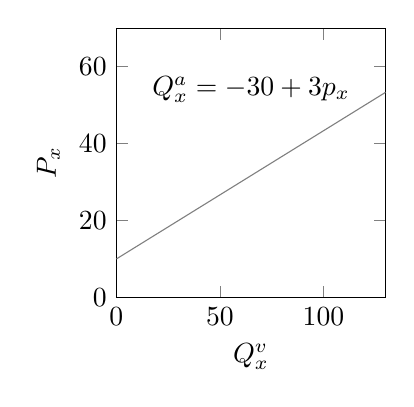
\begin{tikzpicture}
	\begin{axis}[name=left,xlabel=$Q_x^v$, ylabel=$P_x$, ymin=0, xmin=0, xmax=130, ymax=70,width=5cm, height=5cm]
		\addplot[gray, samples=120, domain=0:130] {10+(1/3)*x};
		\draw (axis cs:65,60) node[below]{$Q_x^a=-30+3p_x$};
	\end{axis}
\end{tikzpicture}
\caption{Een parti\"ele aanbodfunctie van een product $x$ bij varierende prijs $P_x$}
\label{fig:h2-aanbodfunctie}
\end{figure}

\par De voorgaande parti\"ele functies kan men in \'e\'en grafiek samen brengen (figuur \ref{fig:h2-marktevenwicht}). De prijs bereikt dan een evenwicht in hun snijpunt (bij $p_x=30$ en $q=60$). Dit noemt men het \entry{marktevenwicht}. Het is een evenwicht dat \textit{automatisch} tot stand komt.
\par Het marktevenwicht is een evenwicht waar de laatst geproduceerde eenheid evenveel opbrengt aan de producent als hij hem kost. Bereiken we geen evenwicht, dan is er \'of een \entry{vraagoverschot}, \'of een \entry{aanbodoverschot}.

\begin{figure}[H]
\vspace{0.5cm}
\centering\small
\captionsetup{justification=centering,margin=2cm}
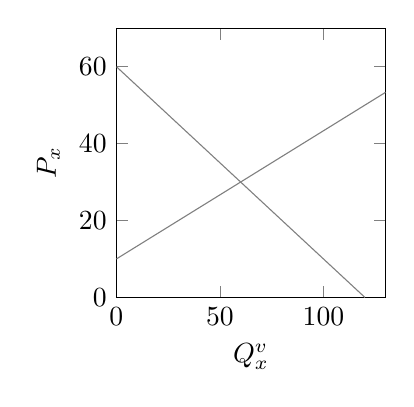
\begin{tikzpicture}
	\begin{axis}[name=left,xlabel=$Q_x^v$, ylabel=$P_x$, ymin=0, xmin=0, xmax=130, ymax=70,width=5cm, height=5cm]
		\addplot[gray, samples=120, domain=0:130] {10+(1/3)*x};
		\addplot[gray, samples=120, domain=0:120] {60-(1/2)*x};
	\end{axis}
\end{tikzpicture}
\caption{Het marktevenwicht}
\label{fig:h2-marktevenwicht}
\end{figure}

Wat door de consumenten moet worden betaald is kleiner dan de totale betalingsbereidheid. Het verschil tussen beide (oppervlakte figuur \ref{fig:h2-surplus}(a)) noemt men het \entry{consumentensurplus}.
\par Voor de producenten noemt men de totale ontvangst min de totale kost het \entry{producentensurplus} (figuur \ref{fig:h2-surplus}(b)).
\par We zien dat er dus spontaan wederzijds voordelige ruil ontstaat. Beter kan niet, want het gezamenlijk surplus is maximaal. Men heeft het over \entrystyled{pareto-efficientie}{Pareto-effici\"entie}. Helaas ontstaat dergelijk evenwicht enkel in de theoretische `volmaakte mededinging' (wij gingen uit van prijsnemerschap en homogene producten ...).

\begin{figure}[H]
\centering
\captionsetup{justification=centering,margin=2cm}
\begin{tikzpicture}
	\begin{axis}[name=left,xlabel=$Q_x^v$, ylabel=$P_x$, ymin=0, xmin=0, xmax=130, ymax=70,width=5cm, height=5cm]
		\addplot[gray, samples=120, domain=0:130] {10+(1/3)*x};
		\addplot[gray, samples=120, domain=0:120] {60-(1/2)*x};
		\addplot[draw=none,pattern=north west lines, pattern color=gray!50!gray] coordinates {(0,30) (60,30) (0,60)};
	\end{axis}
	\begin{axis}[xshift=3cm,at={(left.north east)},anchor=north west,xlabel=$Q_x^v$, ylabel=$P_x$, ymin=0, xmin=0, xmax=130, ymax=70,width=5cm, height=5cm]
		\addplot[gray, samples=120, domain=0:130] {10+(1/3)*x};
		\addplot[gray, samples=120, domain=0:120] {60-(1/2)*x};
		\addplot[draw=none,pattern=north west lines, pattern color=gray!50!gray] coordinates {(0,10) (60,30) (0,30)};
	\end{axis}
\end{tikzpicture}
\caption{Marktevenwicht met in het gearceerd deel het (a) consumentensurplus, \\(b)  producentensurplus}
\label{fig:h2-surplus}
\end{figure}

\subsection{Elasticiteiten}

Stel we hebben een functie $y=f(x)$, met $x$ de verklarende variabele en $y$ de te verklaren variabele. Relatieve (procentuele) veranderingen\footnote{Verandert $x$ van $x_0$ naar $x_1$, dan is de relatieve verandering van $x$ gelijk aan de verandering van $x$ (namelijk $\Delta x=x_1-x_0$) gedeeld door de beginwaarde $x_0$.} in $x$ en $y$ noteert men respectievelijk als $\frac{\Delta x}{x_0}$ en $\frac{\Delta y}{y_0}$. De \entry{boogelasticiteit} van $y$ ten opzichte van $x$ definieert men dan als :

$$E_x^y	 = \frac{\frac{y_1-y_0}{y_0}}{\frac{x_1-x_0}{x_0}}
		 = \frac{\frac{\Delta y}{y_0}}{\frac{\Delta x}{x_0}}
		 = \frac{\Delta y}{\Delta x}\cdot\frac{x_0}{y_0}$$

Het is dus de verhouding van relatieve veranderingen over een bepaalde `boog' van de curve.
\par Willen we de elasticiteit in een bepaald punt berekenen, dan kijkt men eerder naar de infinitesimale verandering op $x$ ($\text{lim}_{\Delta x\rightarrow 0}$). Dit is de \entry{puntelasticiteit} $\epsilon_x^y$, dus een afgeleide (hoofdstuk \ref{sec:appafg}) :\\
$$\epsilon_x^y=(\text{lim}_{\Delta x\rightarrow 0}\frac{\Delta y}{\Delta x})\frac{x}{y}=\frac{dy}{dx}\cdot\frac{x}{y}$$

\par In de economie gebruiken we allerhande elasticiteiten (tabel \ref{tab:h2elas}).

\begin{table}[H]
\small\centering\captionsetup{justification=centering,margin=2cm}
\begin{tabular}{c | c | c | c}
\textbf{Afhankelijke} & \textbf{Onafhankelijke} & \textbf{Naam} & \textbf{Belang}\\
\hline
$Q_x^v$ & $P_x$ & Prijselasticiteit van de vraag & Invloed belastingen en subsidies, marktvormen.\\
$Q_x^a$ & $P_x$ & Prijselasticiteit van het aanbod & Invloed belastingen en subsidies.\\
$Q_x^v$ & $Y$ & Inkomenselasticiteit van de vraag & Normaal (luxe en noodzakelijk) vs. inferieur.\\
$Q_x^v$ & $P_z$ & Kruiselingse prijselasticiteit van de vraag & Complementen en substituten.\\
\end{tabular}
\caption{Elasticiteiten gebruikt in de economie}
\label{tab:h2elas}
\end{table}

Bij de prijselasticiteit van de vraag is $Q_x^v$ (de gevraagde hoeveelheid) de te verklaren variabele. De prijs $p_x$ is de verklarende variabele. Het is een maat voor hoe sterk de prijs de gevraagde hoeveelheid be\"invloedt. De boogelasticiteit is dan :

$$E_{p_x}^{q_x^v}
		 = \frac{\frac{\Delta {q_x^v}}{{q_x^v}_0}}{\frac{\Delta {p_x}}{{p_x}_0}}
		 = \frac{\Delta {q_x^v}}{\Delta {p_x}}\cdot\frac{{p_x}_0}{{q_x^v}_0}$$
		
Voor de vraagfunctie die we in het vorige hoofdstuk gebruikten is de tweede factor gelijk aan de richtingsco\"effici\"ent. De overeenkomstige puntelasticiteit is :
$$\epsilon_{p_x}^{q_x^v}=\frac{d{q_x^v}}{d{p_x}}\cdot\frac{{p_x}}{{q_x^v}}$$
Voorbeelden daarvan zie je in figuur \ref{fig:h2-elasticiteiten}. De rode horizontale as illustreert een perfect elastische vraag ; de vraag kan veranderen zelfs als de prijs niet verandert. Dit in tegenstelling tot de perfect prijs-inelastische, blauwe vraagfunctie. Daar verandert de hoeveelheid nooit, wat de prijs ook is (zoals bij de vraag naar doodskisten).

\begin{figure}[H]
\vspace{0.5cm}
\centering\small
\captionsetup{justification=centering,margin=2cm}
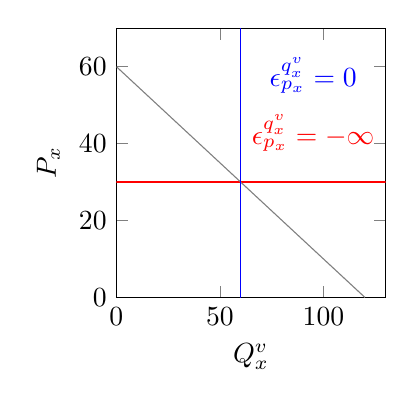
\begin{tikzpicture}
	\begin{axis}[name=left,xlabel=$Q_x^v$, ylabel=$P_x$, ymin=0, xmin=0, xmax=130, ymax=70,width=5cm, height=5cm]
		\addplot[red, samples=120, domain=0:130] {30};
		\addplot[gray, samples=120, domain=0:120] {60-(1/2)*x};
		\addplot +[mark=none,draw=blue] coordinates {(60, -1) (60, 70)};
		\draw[blue] (axis cs:95,65) node[below]{$\epsilon_{p_x}^{q_x^v}=0$};
		\draw[red] (axis cs:95,50) node[below]{$\epsilon_{p_x}^{q_x^v}=-\infty$};
	\end{axis}
\end{tikzpicture}
\caption{Voorbeelden van prijsinelasticiteiten}
\label{fig:h2-elasticiteiten}
\end{figure}

In absolute waarde\footnote{Bij de absolute waarde van een getal laat men het minteken wegvallen.} is de prijselasticiteit des te groter naarmate ...
\begin{itemize}
\item[-] ... er meer substituutgoederen er zijn (dat zie je in volmaakte mededinging).
\item[-] ... de behoefte minder dwingend is (de vraag naar een levensreddend geneesmiddel zal niet elastisch zijn).
\item[-] ... het budgetaandeel groter is (als je een wagen koopt ga je meer kijken naar de prijs dan bij het kopen van paperclips).
\item[-] ... de beschouwde tijdsperiode langer wordt (op korte termijn verliep de aanpassing op verhogende olieprijzen moeizaam, maar na verloop van tijd wierpen energiebesparende technieken hun vruchten af en was er een beduidende daling van het verbruik van olieproducten).
\end{itemize}

We kijken vervolgens naar de inkomenselasticiteit van de vraag : 

$$E_{y}^{q_x^v} = \frac{\Delta {q_x^v}}{\Delta {p_x}}\cdot\frac{{y}_0}{{q_x^v}_0}
\qquad | \qquad
\epsilon_{y}^{q_x^v}=\frac{d{q_x^v}}{d{y}}\cdot\frac{{y}}{{q_x^v}}$$

Dit geeft dus aan in welke mate de inkomst de vraag be\"invloedt. Afhankelijk van het type goed waarnaar gevraagd wordt gaat de elasticiteit positief of negatief zijn. We onderscheiden :
\begin{itemize}
\item[-] \entrystyled{normaal goed}{normale goederen} : $\epsilon_y^V>0$ (consumptie stijgt bij stijgend inkomen).
\item[-] \entrystyled{inferieur goed}{inferieure goederen} : $\epsilon_y^V<0$ (consumptie daalt bij stijgend inkomen).
\item[-] \entrystyled{noodzakelijk goed}{noodzakelijke goederen} : $0<\epsilon_y^V<1$ (consumptie stijgt bij stijgend inkomen, maar het budgetaandeel daalt). Een voorbeeld is voeding.
\item[-] \entrystyled{luxegoed}{luxegoederen} : $1<\epsilon_y^V$ (hoe rijker men wordt, hoe groter het percentage van het budget dat er aan wordt besteed). Voorbeelden zijn wijn, restaurantbezoeken of reizen.
\end{itemize}

Als we het effect van de prijs van \'e\'en product op de gevraagde hoeveelheid van een ander product wil meten, dan gebruikt men de \entry{kruiselingse prijselasticiteit} :

$$E_{p_x}^{q_z^v} = \frac{\Delta {q_z^v}}{\Delta {p_x}}\cdot\frac{{p_x}_0}{{q_z^v}_0}
\qquad | \qquad
\epsilon_{p_x}^{q_z^v}=\frac{d{q_z^v}}{d{p_x}}\cdot\frac{{p_x}}{{q_z^v}}$$

Deze is uiteraard positief bij substituten, zelfs oneindig bij perfecte substituten. Als de prijs van koffie stijgt gaat er bijvoorbeeld meer naar thee gevraagd worden.
\par Bij complementen is de kruiselingse prijselasticiteit negatief, en bij onafhankelijke producten is hij nul.\\

\par Bij vraag- en aanbodschokken (hoofdstuk \ref{sec:h2veas}) zal men ook zien dat de prijselasticiteit van het aanbod van belang is :

$$E_{p_x}^{q_x^a} = \frac{\Delta {q_x^a}}{\Delta {p_x}}\cdot\frac{{p_x}_0}{{q_x^a}_0}
\qquad | \qquad
\epsilon_{p_x}^{q_x^a}=\frac{d{q_x^a}}{d{p_x}}\cdot\frac{{p_x}}{{q_x^a}}$$

Deze prijselasticiteit kan nul zijn. Als de prijs van olie stijgt zal het aanbod niet noodzakelijk stijgen, bijvoorbeeld omdat er niet genoeg is.

\subsection{Vraag- \& Aanbodschokken}\label{sec:h2veas}

Wanneer de vraagfunctie z\'elf naar rechts of naar links verschuift, dan heeft men het over een (respectievelijk positieve of negatieve) \entry{vraagschok}. Een positieve vraagschok verhoogt de vraag en een negatieve vraagschok leidt tot een daling van de vraag.\\

\par In deze context gaat men niet meer vanuit van `\textit{ceteris paribus}'. Positieve vraagschokken (eg. figuur \ref{fig:h2-schok}(a)) kunnen dan teweeg gebracht worden door een stijging van de prijs van een substituut, de daling van de prijs van een complement, de stijging van het aantal consumenten, de stijging van het inkomen, verandering van voorkeuren, een subsidie\index{subsidie}, ... De vraagcurve verplaatst naar rechts, en zowel de evenwichtsprijs als de evenwichtshoeveelheid stijgen. De verhouding van deze stijgingen hangt af van de prijselasticiteit van het aanbod.\\

\par Bij een negatieve aanbodschok (figuur \ref{fig:h2-schok}(b)) schuift de vraagcurve naar links. Dit kan zich voordoen bij de stijging van de lonen, stijging van de vergoeding van het kapitaal, daling van het aantal bedrijven, daling van de productiviteit, een belasting\index{belasting}, ...
\par En dan gaat de evenwichtshoeveelheid dus dalen en de evenwichtsprijs stijgen. De verhouding tussen deze veranderingen hangt af van de prijselasticiteit van de vraag.

\begin{figure}[H]
\centering
\captionsetup{justification=centering,margin=2cm}
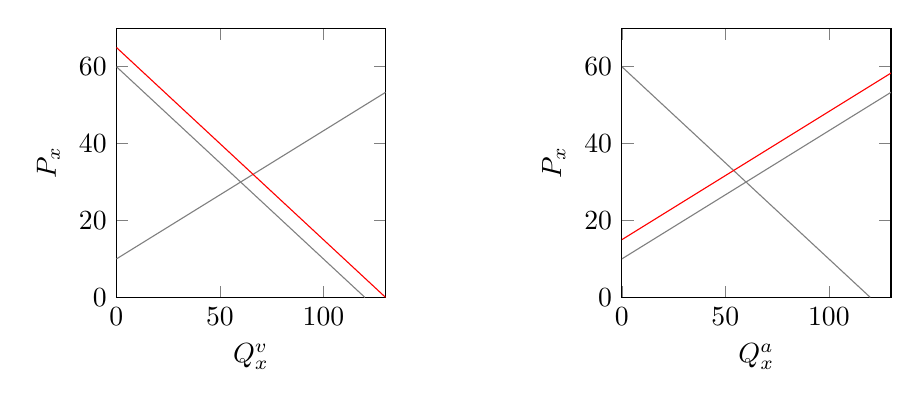
\begin{tikzpicture}
	\begin{axis}[name=left,xlabel=$Q_x^v$, ylabel=$P_x$, ymin=0, xmin=0, xmax=130, ymax=70,width=5cm, height=5cm]
		\addplot[gray, samples=120, domain=0:130] {10+(1/3)*x};
		\addplot[gray, samples=120, domain=0:120] {60-(1/2)*x};
		\addplot[red, samples=120, domain=0:130] {65-(1/2)*x};
	\end{axis}
	\begin{axis}[xshift=3cm,at={(left.north east)},anchor=north west,xlabel=$Q_x^a$, ylabel=$P_x$, ymin=0, xmin=0, xmax=130, ymax=70,width=5cm, height=5cm]
		\addplot[gray, samples=120, domain=0:130] {10+(1/3)*x};
		\addplot[gray, samples=120, domain=0:120] {60-(1/2)*x};
		\addplot[red, samples=120, domain=0:130] {15+(1/3)*x};
	\end{axis}
\end{tikzpicture}
\caption{(a) Positieve vraagschok, \\(b) Negatieve aanbodschok}
\label{fig:h2-schok}
\end{figure}

\subsection{Belastingen \& Subsidies}

We merkten eerder op dat schokken kunnen veroorzaakt worden door \glslink{belasting}{belastingen}\index{belasting} (op het inkomen of de consumptie) en \glslink{subsidie}{subsidies}\index{subsidie} (eigenlijk belastingsaftrek).\\

\par Stel, we passen een \textit{belasting op de producent} toe. Dit geeft een negatieve aanbodschok. De prijs verhoogt dus. Wie betaalt de prijs dan?
\par Als de belasting 5 euro per product bedraagt, dan stijgt de prijs niet noodzakelijk met 5. Als de vraagvergelijking bijvoorbeeld $Q_x^v=120-2\cdot p_x$ is, en de aanbodvergelijking $Q_x^a=-30+3\cdot p_x$, dan wordt de aanbodvergelijking met de belasting $Q_x^a=-30+3\cdot(p_x-5)$ en bereikt men een evenwicht in $p_x=33,q=54$ (figuur \ref{fig:h2-schok}(b)). De producentenprijs (wat de producent krijgt voor elk product) wordt dus $p_a=33-5=28$ (door de belasting), en de consumentenprijs (wat de consument betaalt) wordt $p_v=33$. Het is de consument die meer betaalt! 
\par Wie het meeste betaalt hangt dus af van de elasticiteiten (voor de vergelijkingen de richtingsco\"effici\"enten). Als de vraag in ons voorbeeld perfect inelastisch zou zijn (verticale vraagcurve), dan zou de consument alles betalen.\\

\par Een \textit{belasting op de consument} gebeurt analoog. Dit geeft een negatieve vraagschok (de vraagcruve schuift naar links, zie figuur \ref{fig:h2-schok2}(a)), want plots is de consument minder bereid te betalen.

\begin{figure}[H]
\centering
\captionsetup{justification=centering,margin=2cm}
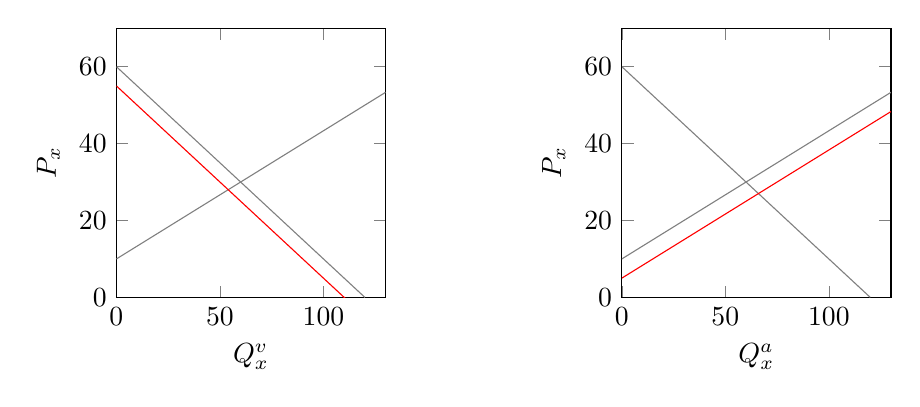
\begin{tikzpicture}
	\begin{axis}[name=left,xlabel=$Q_x^v$, ylabel=$P_x$, ymin=0, xmin=0, xmax=130, ymax=70,width=5cm, height=5cm]
		\addplot[gray, samples=120, domain=0:130] {10+(1/3)*x};
		\addplot[gray, samples=120, domain=0:120] {60-(1/2)*x};
		\addplot[red, samples=120, domain=0:130] {55-(1/2)*x};
	\end{axis}
	\begin{axis}[xshift=3cm,at={(left.north east)},anchor=north west,xlabel=$Q_x^a$, ylabel=$P_x$, ymin=0, xmin=0, xmax=130, ymax=70,width=5cm, height=5cm]
		\addplot[gray, samples=120, domain=0:130] {10+(1/3)*x};
		\addplot[gray, samples=120, domain=0:120] {60-(1/2)*x};
		\addplot[red, samples=120, domain=0:130] {5+(1/3)*x};
	\end{axis}
\end{tikzpicture}
\caption{(a) Negatieve vraagschok, \\(b) Positieve aanbodschok}
\label{fig:h2-schok2}
\end{figure}

De evenwichtshoeveelheid daalt, de prijs ook. Nemen we hetzelfde voorbeeld als in vorige paragraaf, dan wordt het evenwicht deze keer bereikt bij $p_x=28,q=54$, met $p_v=28+5=33$ en $p_a=28$. De consument is dus degene die de belasting voornamelijk betaalt, maar de consument ziet er ook van af (de verhouding hangt weer af van de prijselasticiteiten).\\

\par\noindent Belastingen hebben een aantal kenmerken ; ze zijn \entry{marktconform}, dat wil zeggen, ze staan de gelijkheid van de aangeboden en gevraagde hoeveelheid niet in de weg.
\par De legale belastingplichtige, zoals we eerder zagen, draagt ook niet de volledige last van de belasting. Hij wentelt een deel van de belasting af op de consumenten of producenten. De mate van afwenteling hangt af van de prijselasticiteiten (richtingsco\"effici\"enten) van de vraag en het aanbod. Hoe \textit{groter} de elasticiteit, hoe voordeliger de belasting gaat zijn voor de betrokken partij.\\

\par We kunnen dezelfde redenering toepassen op subsidies aan de consument of producent. En dan hebben we te maken met een positieve vraagschok en een positieve aanbodschok. 
\par Een subsidie van 5 euro aan de consument maakt onze vraagvergelijking $Q_x^v=120-2\cdot(p_x-5)$. Het evenwicht wordt bereikt in $p=32,q=66$, met $p_a=32$ en $p_v=27$. Het is de consument die het meeste wint.
\par Een subsidie van 5 euro aan de producent maakt onze aanbodvergelijking $Q_x^a=-30+3\cdot(p_x+5)$. Het evenwicht wordt bereikt in $p=32,q=66$, met $p_a=32$ en $p_v=27$. Het is de producent die het meeste wint.
\par Bij subsidies wil de betrokken partij dus - in tegenstelling tot bij belastingen - \textit{minder} prijselastischer zijn! Want dan verdient hij er meer aan.\\

\par Subsidies zijn ook marktconform, en wie de subsidie krijgt, krijgt ze niet volledig. De verhouding (welke partij het meeste van de subsidie geniet) hangt, net zoals bij de belastingen, af van de prijselasticiteit. Hoe \textit{kleiner} de elasticiteit, hoe voordeliger de subsidie gaat zijn voor de betrokken partij.

\subsection{Prijsregulering \& Quota's}

Naast de belastingen en subsidies zijn er ook andere maatregelen die gebruikt kunnen worden. Zo heb je de \entry{bindende maximumprijs} of de \entry{bindende minimumprijs} (figuur \ref{fig:h2-quota}).\\

\par Stel, de overheid legt een maximumprijs op voor de huur van appartementen. Bij deze bindende\footnote{`Bindend' verwijst naar het feit dat de maximumprijs kleiner is dan de evenwichtsprijs.} maximumprijs ontstaat een \entry{vraagoverschot} (meer consumenten zijn ge\"interesseerd in een appartement aan 1500 in plaats van 2000 euro). Dit kan aangekaart worden via \entry{rantsoenering}\footnote{Bij prestigieuze scholen zie je soms ouders kamperen voor de school. Deze rantsoenering is dus van de vorm `\textit{eerst komt, eerst waart}'.}, wat betekent dat je de prijs perfect inelastisch maakt (verticale blauwe lijn figuur \ref{fig:h2-quota}(a)). Je kapt in feite de vraag af.
\par Bij een bindende maximumprijs op het aanbod neemt het aanbod ook af (de kosten zijn te hoog voor vele aanbieders), wat artificieel opgekrikt kan worden (horizontale blauwe lijn figuur \ref{fig:h2-quota}(a)). Zo zal de overheid bijvoorbeeld sociale woningen beschikbaar maken.

\begin{figure}[H]
\centering
\captionsetup{justification=centering,margin=2cm}
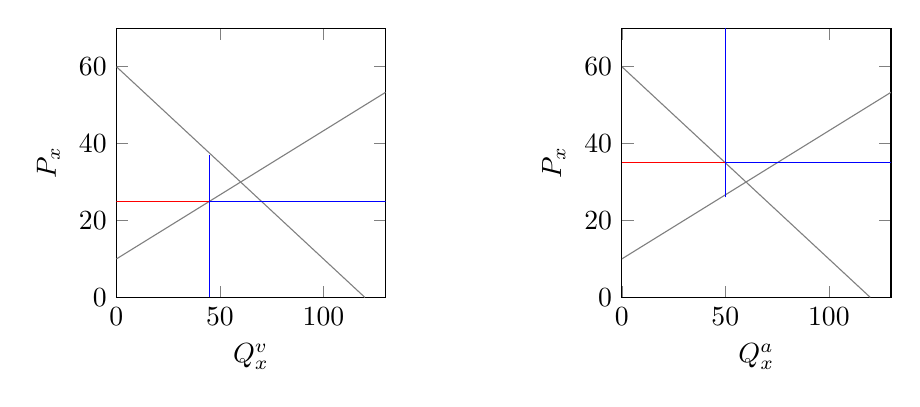
\begin{tikzpicture}
	\begin{axis}[name=left,xlabel=$Q_x^v$, ylabel=$P_x$, ymin=0, xmin=0, xmax=130, ymax=70,width=5cm, height=5cm]
		\addplot[gray, samples=120, domain=0:130] {10+(1/3)*x};
		\addplot[gray, samples=120, domain=0:120] {60-(1/2)*x};
		\addplot[red, samples=45, domain=0:45] {25};
		\addplot[blue] coordinates {(45,0) (45,37)};
		\addplot[blue] coordinates {(45,25) (130,25)};
	\end{axis}
	\begin{axis}[xshift=3cm,at={(left.north east)},anchor=north west,xlabel=$Q_x^a$, ylabel=$P_x$, ymin=0, xmin=0, xmax=130, ymax=70,width=5cm, height=5cm]
		\addplot[gray, samples=120, domain=0:130] {10+(1/3)*x};
		\addplot[gray, samples=120, domain=0:120] {60-(1/2)*x};
		\addplot[red, samples=50, domain=0:50] {35};
		\addplot[blue] coordinates {(50,26) (50,70)};
		\addplot[blue] coordinates {(50,35) (130,35)};
	\end{axis}
\end{tikzpicture}
\caption{(a) Bindende maximumprijs, \\(b) Bindende minimumprijs}
\label{fig:h2-quota}
\end{figure}

Om producenten te beschermen kan de overheid ook een bindende minimumprijs opleggen. Dan ontstaat er een \entry{aanbodoverschot}, wat men kan oplossen door de productie in te perken met productiequota's (figuur \ref{fig:h2-quota}(b), verticale blauwe lijn) of door de vraag artificieel op te krikken (figuur \ref{fig:h2-quota}(b), horizontale blauwe lijn). Bij dit laatste wordt alles via \entrystyled{steunaankoop}{steunaankopen} opgekocht door de staat. Dat kost veel, en houdt vaak in dat men de aangekochte goederen moet vernietigen, dumpen, of bijvoorbeeld verkopen op de wereldmarkt (waar de prijzen dan kunnen dalen) ...\\

\par Het spreekt voor zich dat prijsreguleringen en quota's \textit{niet} \entry{marktconform} zijn.